\documentclass[a4paper,11pt]{article}

\usepackage{url}
\usepackage{graphicx}
\usepackage{enumerate}
\usepackage{amsmath}
\usepackage{float}
\usepackage{longtable}
%\usepackage{fullpage}
\usepackage{pstricks}
\usepackage{tikz}
\usepackage[absolute]{textpos}
\usepackage{import}
\usepackage{subfigure}
\usepackage{setspace}

\title{G54MDP Individual Report}
\author{Marcus Whybrow (mxw18u)} \date{\today}

% Dutch style paragraph formatting
\setlength{\parskip}{1.3ex plus 0.2ex minus 0.2ex}
\setlength{\parindent}{0pt}

%\doublespacing
\onehalfspacing

\begin{document}
	\maketitle
	
	\section{Introduction}
	
	The application which we have created is written for the iOS platform and aims to offer the unified inbox feature of the stock mail app in the guise of an RSS reader.
	
	Choosing a type of app to develop was not easy, and the four of us - Rob Golding, Rob Miles, Michal Konturek and myself - initially were in contention between developing a multi-device multiplayer pong style game and a more standard concept such as an RSS reader.
	
	Additionally there was much debate around the chosen platform, swinging from Android to iOS, back to Android and then finally back to iOS where it was solidified for before development began.
	
	Once we had decided upon creating a ``get out of your way" RSS reader application, the animation and user interaction paradigms available (and out in the wild) within iOS apps offered too much of a benefit over Android, and the decision to develop an iOS app was made.
	
	RSS feeds are a documents which websites provide, defining a list of pages within the website. Each page in the feed is represented by a list of required and optionally defined attributes such as page URL, title and description. An RSS document would typically list the 10 newest pages added to a website, allowing RSS readers to request the document and obtain a list of links and descriptions of the 10 latest items.
	
	Our application entitled ``FeedReader" aims to allow users to keep up to date with the various RSS feeds which they follow by allowing users to track RSS feeds. For each feed, it keeps track of which items have already been read, and allows old items to be deleted once finished with. Each tracked feed can be refreshed - which requests the respective RSS document again - allowing any new items found to be added to the app.
	
	\section{The Concept and Technologies}
	
	Before starting the development of our own feed reading application, we took a look at what was out their already on the App Store. An app named ``Pulse"\footnote{\texttt{http://itunes.apple.com/us/app/pulse-news-reader/id371088673}} seemed to be developed to a high standard and we started to list what we did and did not want in respect to that app.
	
	When Michal first showed us \emph{Pulse} we liked it but though it was too complicated, instead I personally wanted an application which allowed me to know that I had seen all of the the latest posts for the websites which I follow, something akin to being able to tick them off when read, with new items appearing at the top of a list.
	
	At this point I proposed the concept of a unified inbox feature as seen in the stock \emph{mail} application which ships with any new iOS device. Users would be able to see all of the items from various website feeds in one list, and ensure that they had read them all or just delete them from the list if needed.
	
	The \emph{Pulse} application uses a bespoke internet service which the same developers created. This allows them to offload most of the hard work of parsing a variety of feed types onto a server elsewhere, and deliver only the content necessary to the iOS app in a reduced and reliable format. RSS is defined in XML, which tricky to parse and may not even be valid, rather than handle this within our app, we wanted something similar to what the Pulse developers had created. We knew we some sort of middle-man approach might would be necessary between our app and the RSS feed itself. But on the the other hand creating such a service would have been a lot of work which would not have been directly related to the content of this module.
	
	Luckily the research of Rob golding and Rob Miles turned up an interesting find. The Google Feed API\footnote{\texttt{http://code.google.com/apis/feed/}} is a web service accessed via HTTP where the URL of an RSS feed can be given as input and a predictable JSON version of that data is returned.
	
	Michal explained that JSON parsing was easily achieved on iOS devices, and - as apposed to parsing and handling raw RSS XML - this service was used within our application.
	
	\section{Personal Contribution}
	
	Within the group, myself and Michal Konturek were the only 2 members to directly own apple hardware and the Mac OS required to develop an iPhone app. Michal already had experience developing iOS applications at his place of employment whereas I had none. To remedy this shortfall, and to contribute to the project I decided to get up to scratch by offering to create a prototype iOS application which featured only the different screens and ways to navigate between them. The development of this prototype can be seen in the public repository\footnote{\texttt{https://github.com/G54MDP/feedreader}} and encompasses all commits up until commit \verb!4f1794!\footnote{\texttt{https://github.com/G54MDP/feedreader/commit/4f1794}}
	
	\begin{figure}[t]
		\centering
		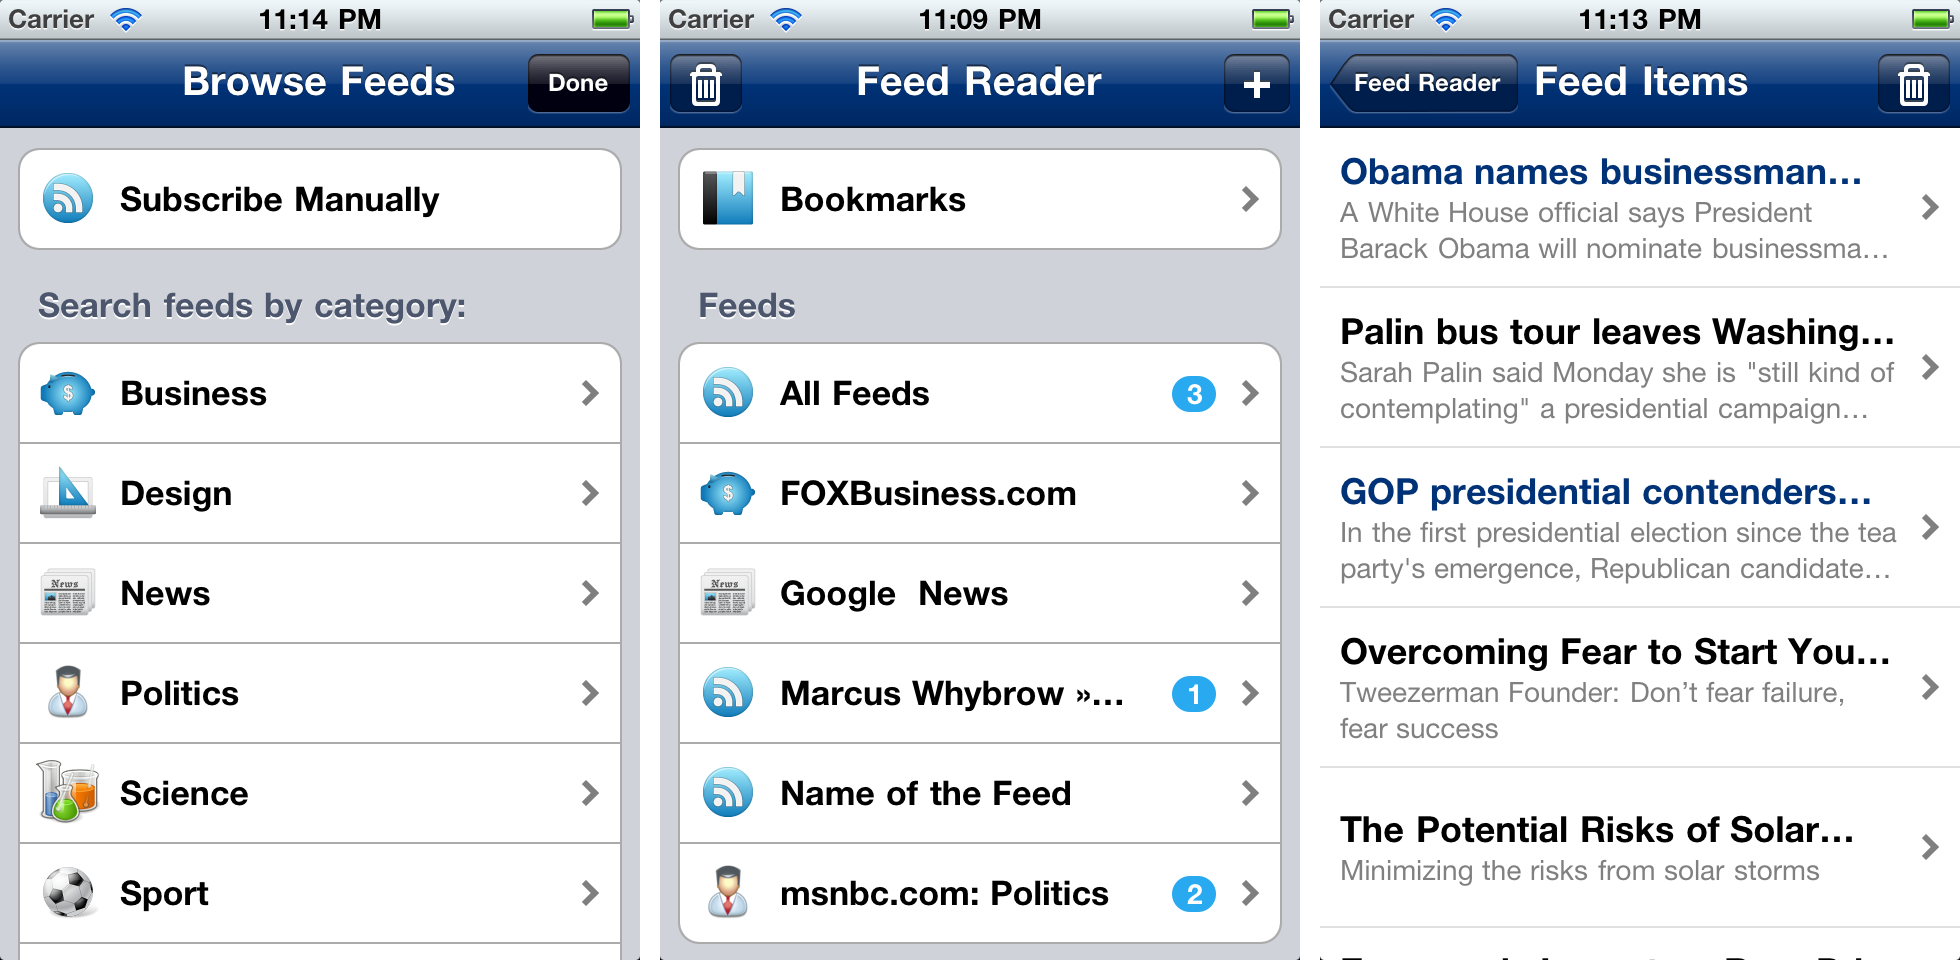
\includegraphics[width=12.65cm]{images/screens1.png}
		\caption{New Feed, feeds and feed screens from left to right.}
		\label{screens1}
	\end{figure}
	
	\begin{figure}[t]
		\centering
		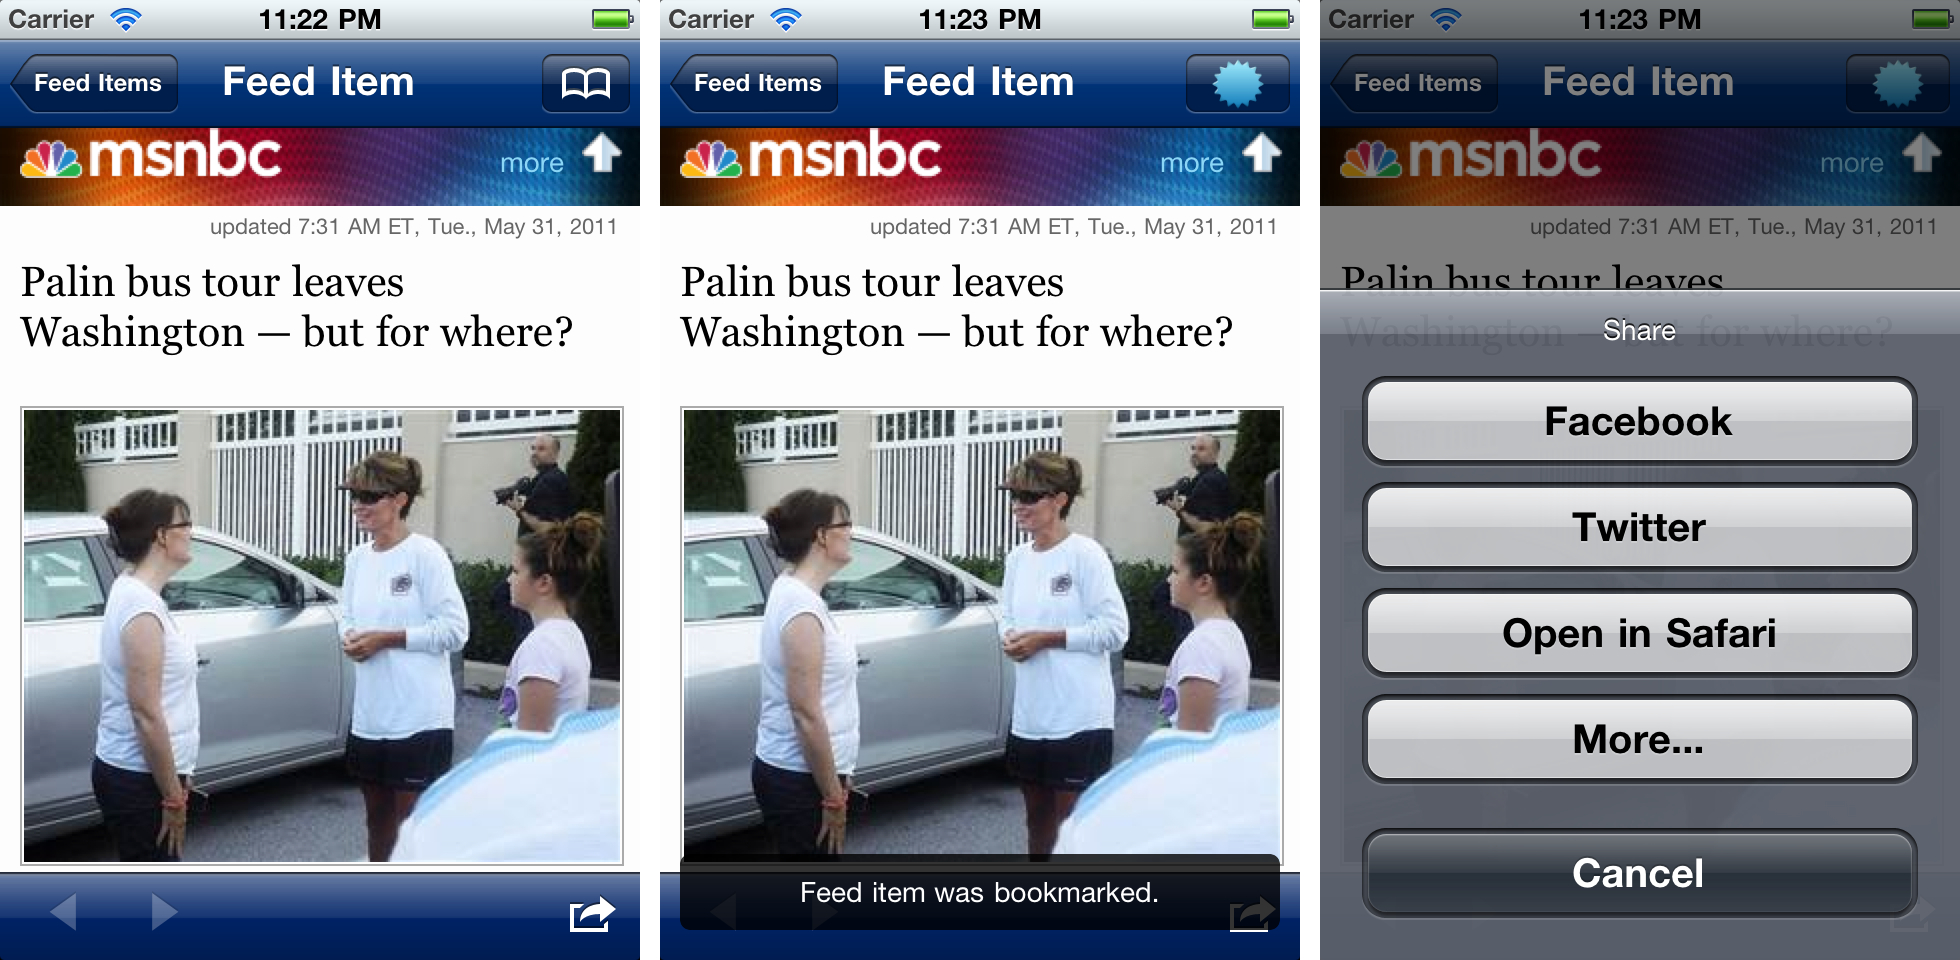
\includegraphics[width=12.65cm]{images/screens2.png}
		\caption{Normal content view, bookmarked item, and sharing menu screens.}
		\label{screens2}
	\end{figure}
	
	Throughout the project I took charge of designing the user interface. The aim was always to be as simple as possible for everyday use, give direct access to the content of each feed item and be simple for new users to pick up. Figure \ref{screens1} shows the main screens which the user will interact with, however the user will spend most of their time in the Feed items view, often opening an closing the app whilst remaining completely within that view or one of its child views.
	
	We expect the user to spend most of their time in the ``All Feeds" section which is similar to the unified inbox approach of the mail app. From this list they can select an individual item to go straight to the URL for that item which is shown in a built in safari view showing in figure \ref{screens2}, this screen has a bookmark button for saving content for later on, but more importantly a sharing button in the bottom right which allows the user to share the URL to this page via various services.
	
	Originally we wanted Twitter and maybe Facebook integration for sharing content from the app, my research revealed a library called ShareKit\footnote{\texttt{http://getsharekit.com/}} which is listed in the officially recommended twitter Objective C libraries. ShareKit provides the ability to share links, images, text or files with a smattering of popular services, including both Twitter and Facebook. Some, such as Facebook and Twitter required registering for access API keys which I gathered for use within the application.
	
	\section{The Group}
    
	After the coursework was announced and the group was formed, we agreed to have regular weekly meetings to make decisions, I do not think that the other groups members would mind me saying that reservations existed regarding particular technologies and areas of interest. For example the contentions between a game and a standard UI based app, and the decisions around Android and iOS. However this was only the manifestation of enthusiasm, and as a whole, we came to agreements using analysis and reason of our situation.
	
	Each member of our group is an accomplished programmer in their own right, and each of us could have made good progress in any of the areas required to make an application of this kind. In fact most decisions where made via a democratic method involving all members, but defaulting to individuals with particular expertise in the relevant subject, whether it be interface design or technical limitations of a platform.
	
	\section{Conclusion}
	
	

\end{document}
